\begin{enumerate}[label=\thesubsection.\arabic*.,ref=\thesubsection.\theenumi]
\numberwithin{equation}{enumi}

\item Find the peak overshoot for the second order control system given by:

\begin{align}
    G(S) = \frac{100}{s^2 + 10s +100}
\end{align}

\solution  The step response is
\begin{align}
    \implies C(S) &= \frac{100}{s\brak{s^2 + 10s +100}}
\end{align}
From the Final Value theorem
\begin{align}
    \lim_{s \to 0} sC(s) = \lim_{t \to \infty} c(t) = 1
\end{align}
%
and by taking the inverse laplace transform
\begin{align}
    c(t) = 1 - \frac{2e^{-5t}}{\sqrt{3}}.\sin \brak{5\sqrt{3}t + \frac{\pi}{3}}
    \label{eq:eebtech11045_ct}
\end{align}


At $t_p$, $c(t)$ is maximum if
\begin{align}
    c'(t)|_{t=t_p} &= 0
\\
\implies      t_p &= \frac{n\pi}{5\sqrt{3}}, \quad n = 1
\\
&= \frac{\pi}{5\sqrt{3}}
\end{align}
%
after some algebra.
From \eqref{eq:eebtech11045_ct} 
\begin{align}
    c\brak{t_p} &= 1 + e^\frac{-\pi}{\sqrt{3}} 
\\
\implies     c\brak{t_p}  -     c\brak{\infty} &= e^\frac{-\pi}{\sqrt{3}} 
\\
&=0.163
\end{align}
%
which is the peak overshoot.  The following code illustrates this in Fig.     \ref{fig:ee18btech11045_fig1}


\begin{lstlisting}
codes/ee18btech11045.py
\end{lstlisting}

\begin{figure}[!h]
    \centering
    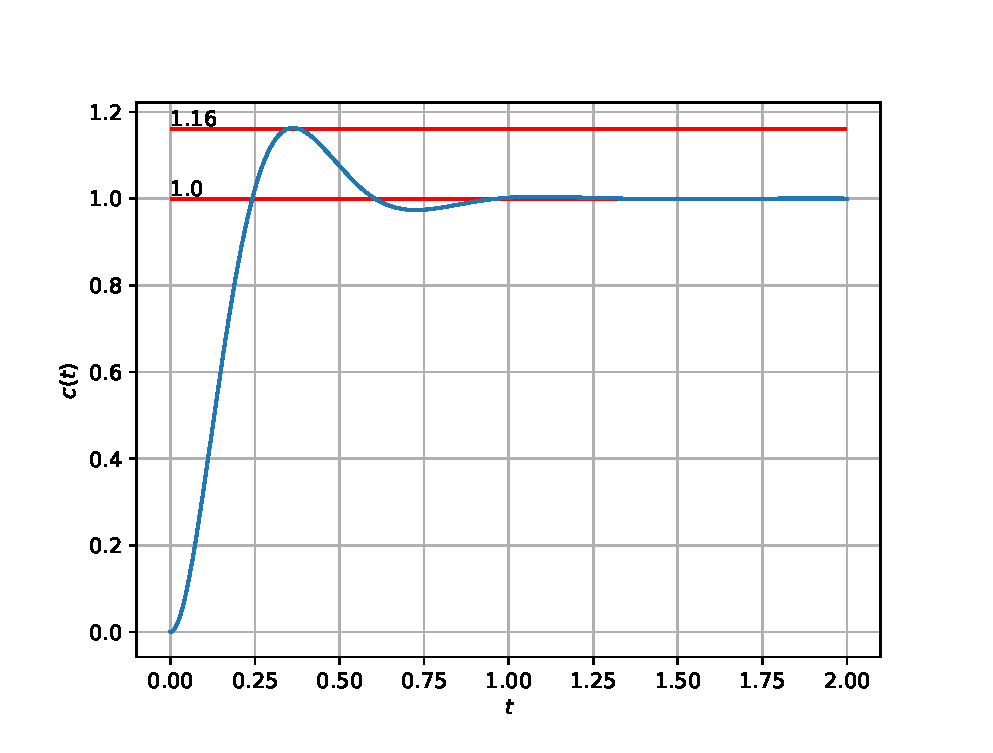
\includegraphics[width=\columnwidth]{figs/ee18btech11045.eps}
    \caption{}
    \label{fig:ee18btech11045_fig1}
\end{figure}

\end{enumerate}
